\section{Durchführung}
\subsection{Versuchsaufbau}
Der Aufbau des Versuchs kann anhand der Fotos in Abb.\ref{fotosaufbau1} bis Abb.\ref{fotosaufbau3} nachvollzogen werden.
\begin{figure}[H]
  \centering
  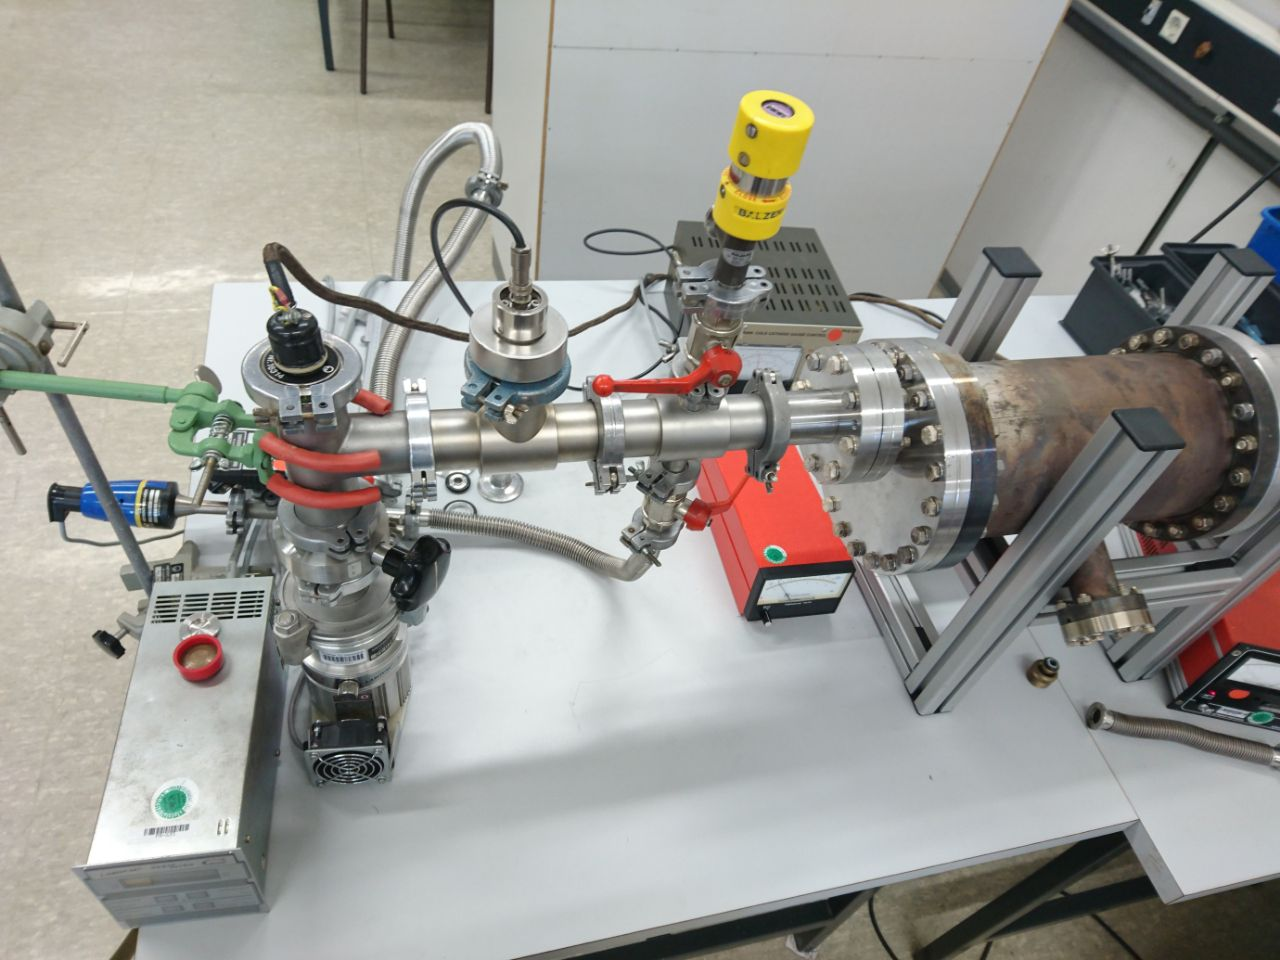
\includegraphics[scale=0.2]{Bilder/Versuch1.jpg}
  \caption{Foto des genutzten Versuchaufbaus.}
  \label{fotosaufbau1}
\end{figure}

\begin{figure}[H]
  \centering
  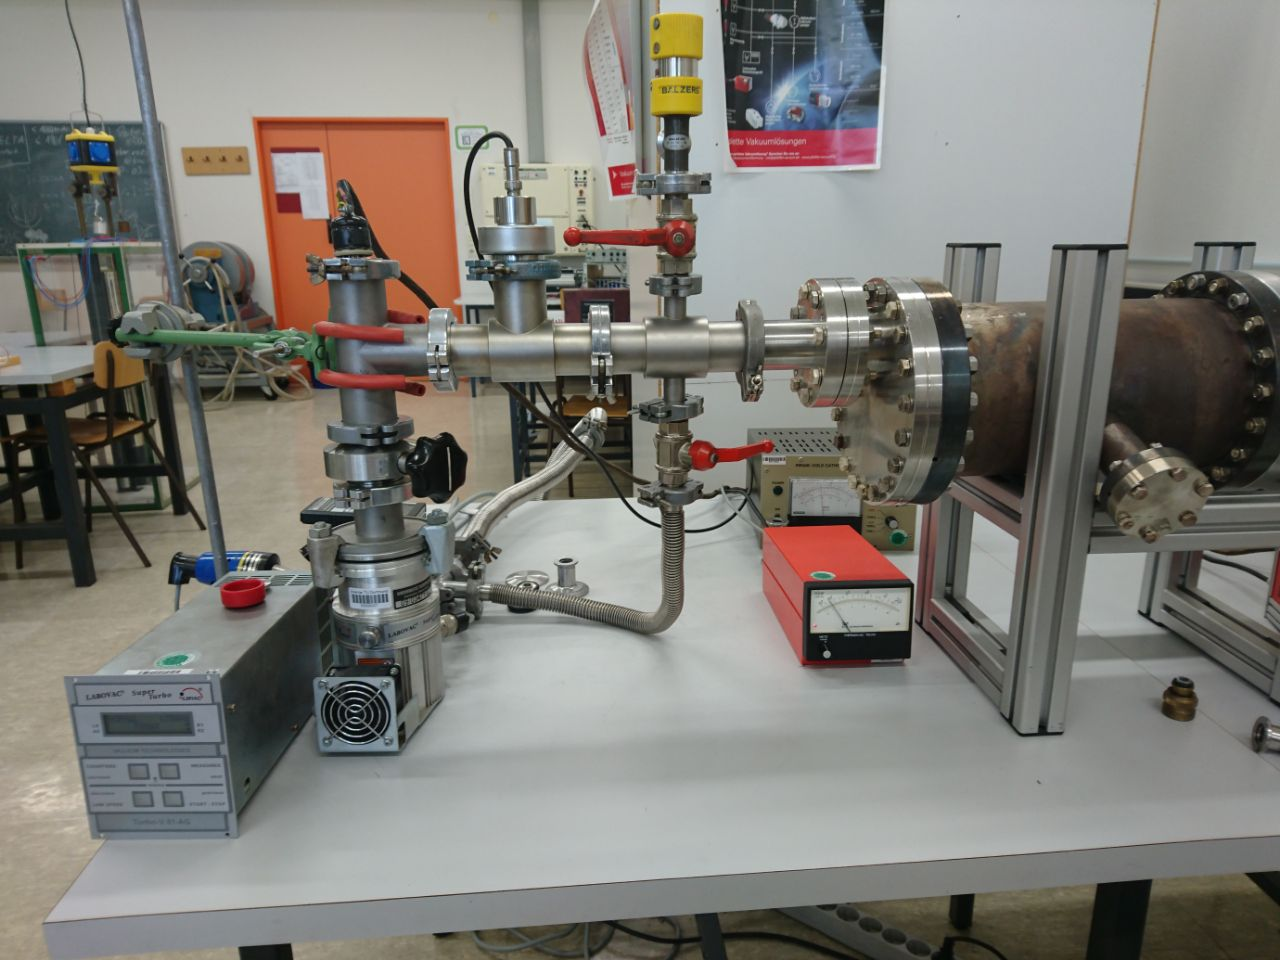
\includegraphics[scale=0.2]{Bilder/Versuch2.jpg}
  \caption{Frontansicht des Versuchaufbaus.}
  \label{fotosaufbau1}
\end{figure}

\begin{figure}[H]
  \centering
  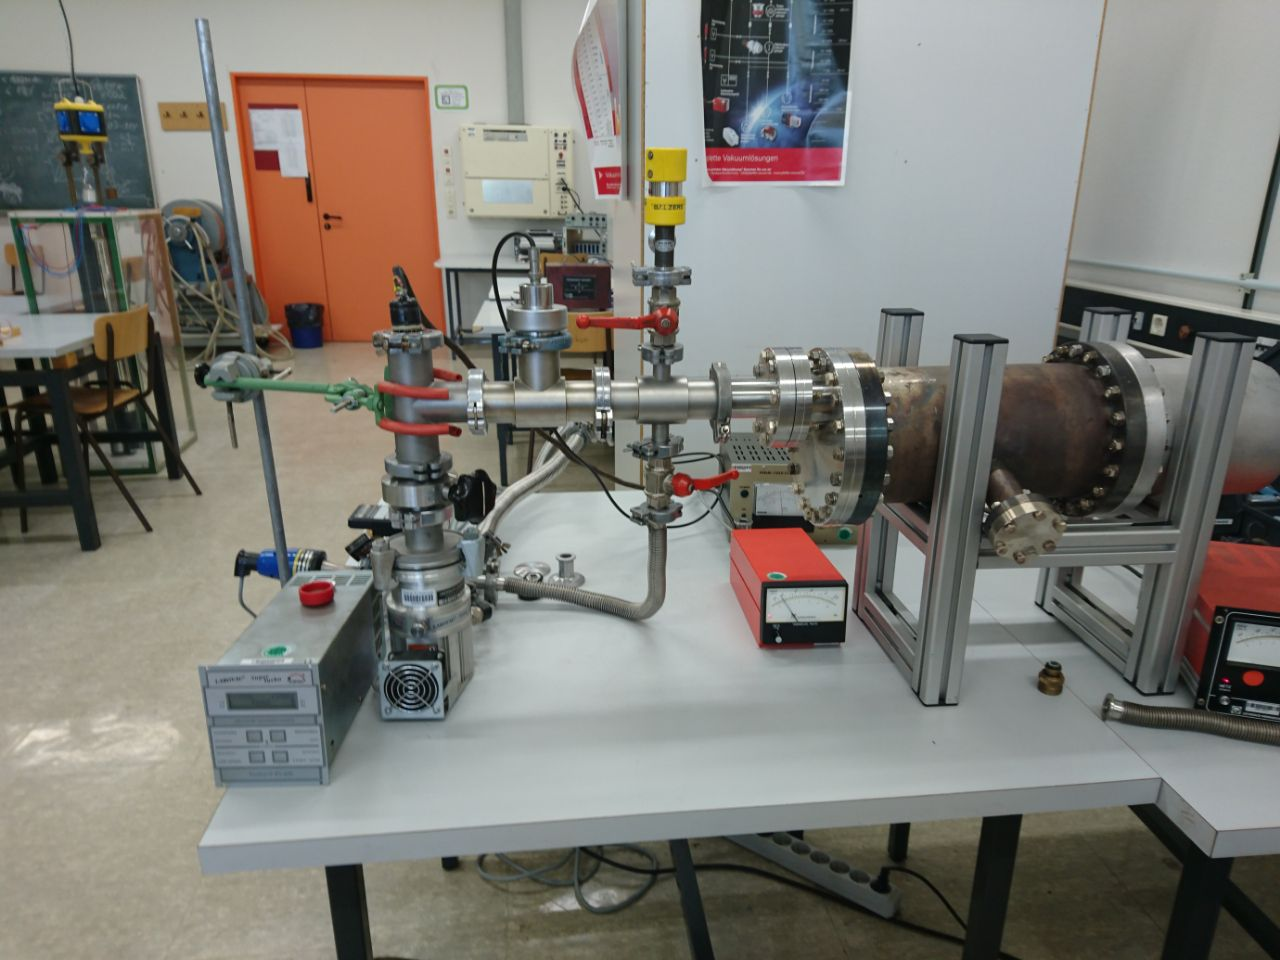
\includegraphics[scale=0.2]{Bilder/Versuch3.jpg}
  \caption{Rückansicht des Aufbaus.}
  \label{fotosaufbau1}
\end{figure}
Zur besseren übersicht findet sich desweiteren in Abb.\ref{aufbauschema} ein schematischer Aufbau des Versuchs.
\begin{figure}[H]
  \centering
  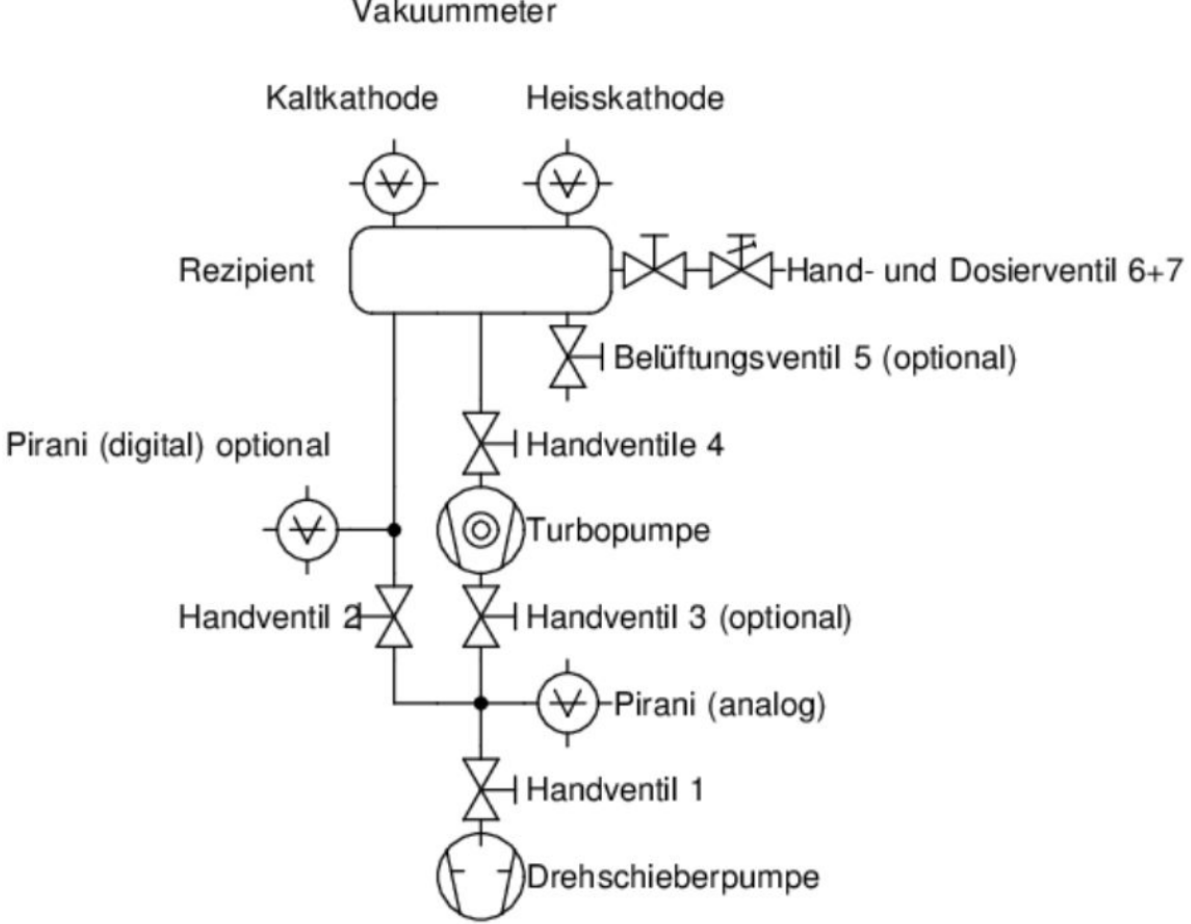
\includegraphics[scale=0.4]{Bilder/schemaVersuch.png}
  \caption{Schematische Darstellung des Versuchsaufbaus. \cite{online}}
  \label{aufbauschema}
\end{figure}
